\documentclass{article}
\usepackage[margin=0.5in]{geometry}
\usepackage{tikz}
\usetikzlibrary{arrows.meta, positioning, shapes.geometric, fit, calc, decorations.pathreplacing}
\usepackage{xcolor}
\usepackage{amssymb}
\usepackage{graphicx}
\pagestyle{empty}

\definecolor{produce}{HTML}{4CAF50}
\definecolor{comm}{HTML}{2196F3}
\definecolor{trade}{HTML}{FF9800}
\definecolor{consume}{HTML}{9C27B0}
\definecolor{spoil}{HTML}{795548}
\definecolor{honest}{HTML}{1565C0}
\definecolor{troll}{HTML}{D32F2F}
\definecolor{mediator}{HTML}{7B1FA2}
\definecolor{lightbg}{HTML}{F5F5F5}

\begin{document}
\thispagestyle{empty}

% ── DIAGRAM 1: Agent Trade Interaction (Chat Style) ──
\resizebox{\textwidth}{!}{%
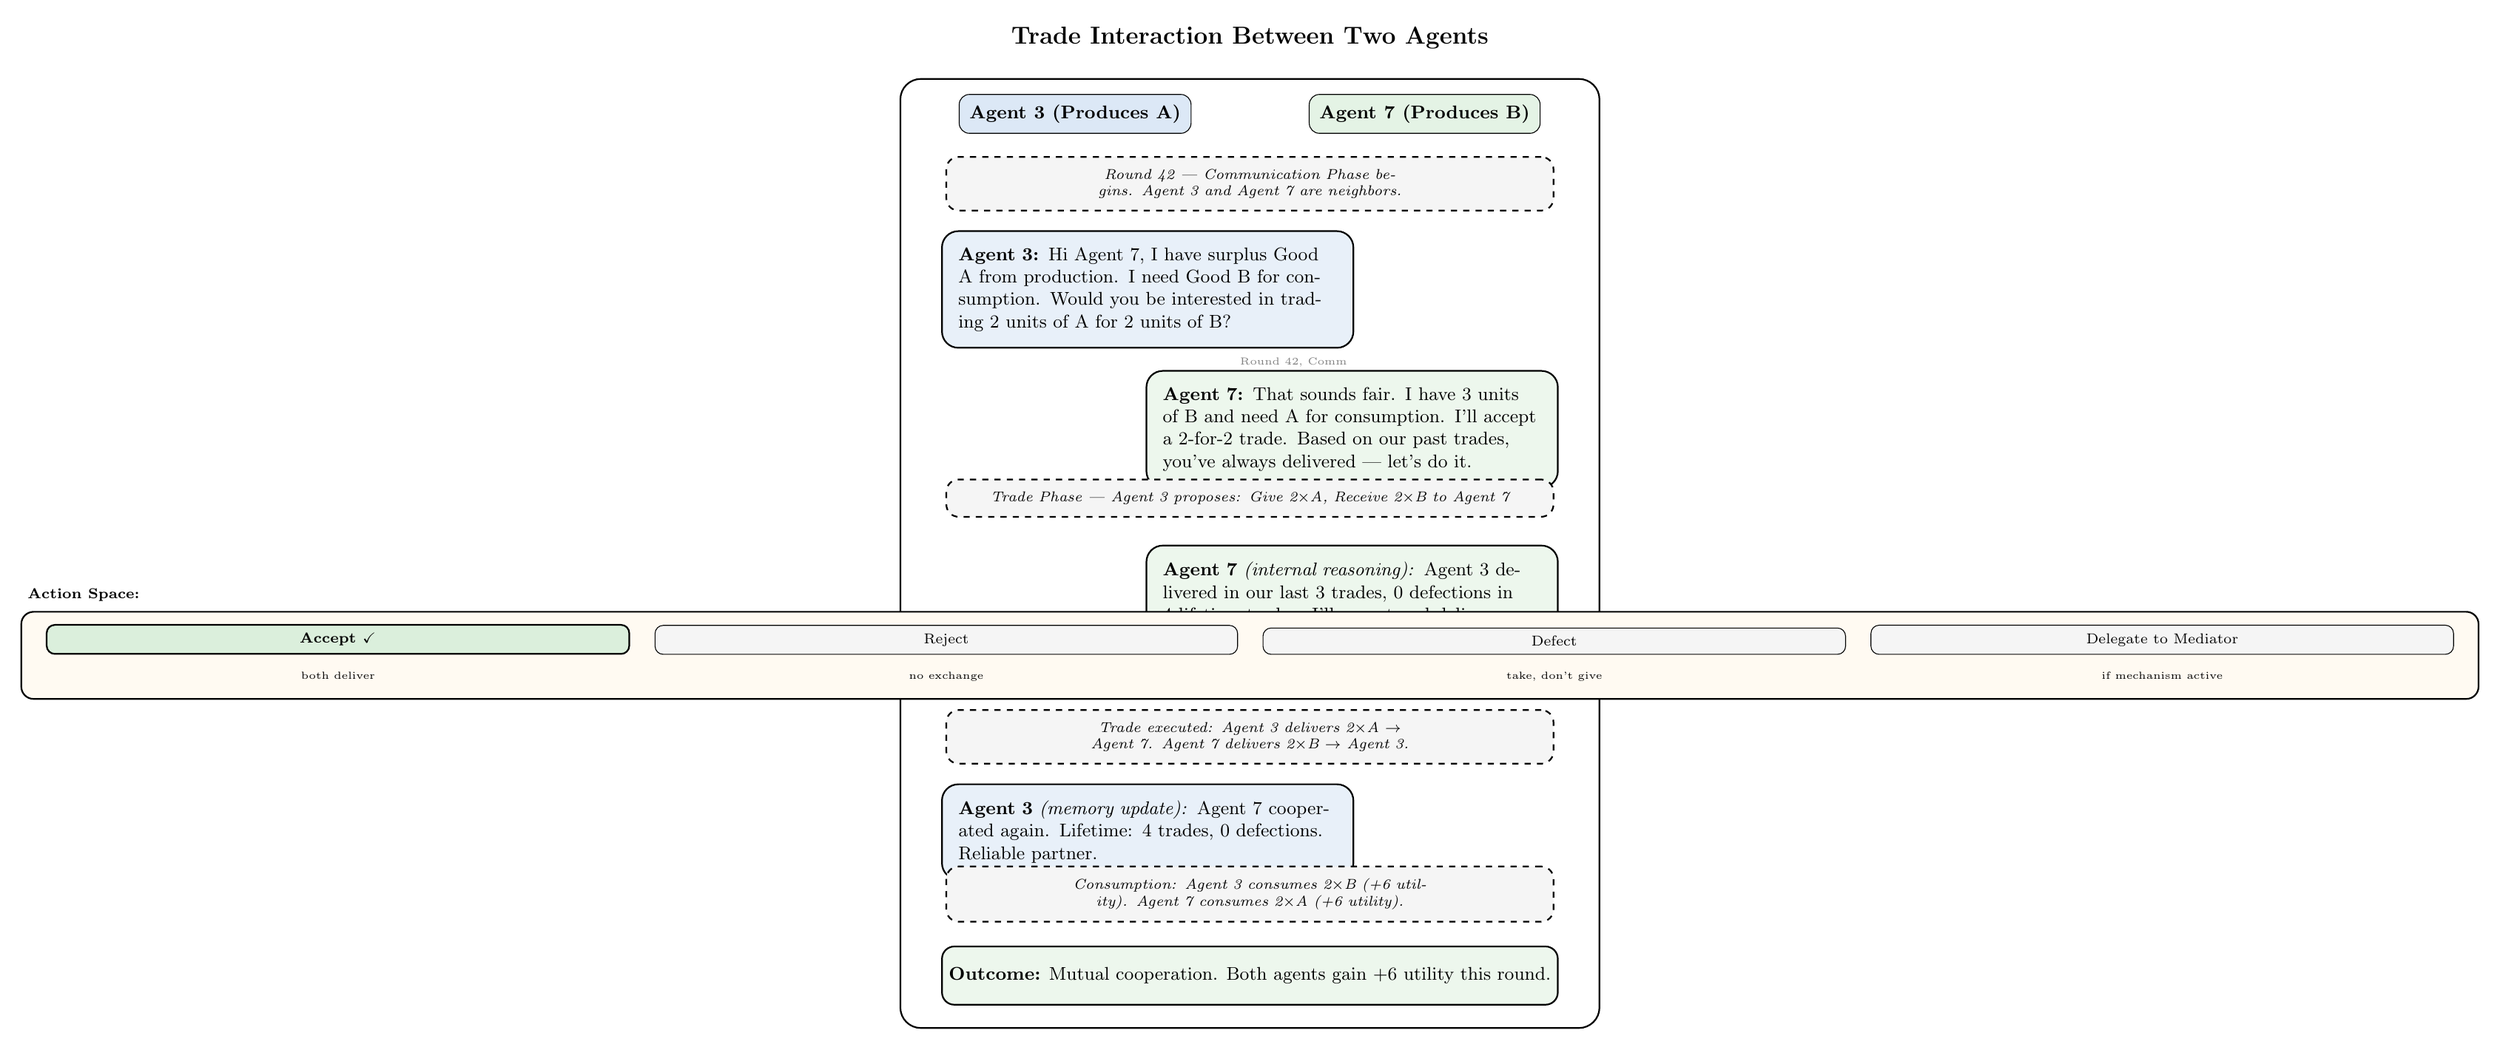
\begin{tikzpicture}[
    bubble left/.style={draw, rounded corners=8pt, fill=honest!10, text width=6.5cm, font=\small, align=left, thick, inner sep=8pt},
    bubble right/.style={draw, rounded corners=8pt, fill=produce!10, text width=6.5cm, font=\small, align=left, thick, inner sep=8pt},
    system/.style={draw, rounded corners=6pt, fill=gray!8, text width=10cm, font=\scriptsize\itshape, align=center, thick, dashed, inner sep=6pt},
    agent label/.style={font=\scriptsize\bfseries, #1},
    timestamp/.style={font=\tiny, gray},
]

% Title
\node[font=\large\bfseries] at (5.5, 16.5) {Trade Interaction Between Two Agents};

% Chat container
\draw[thick, rounded corners=10pt, fill=white] (-0.5, -0.5) rectangle (11.5, 15.8);

% Agent headers
\node[draw, rounded corners=5pt, fill=honest!15, minimum width=3cm, font=\small\bfseries, inner sep=5pt] at (2.5, 15.2) {Agent 3 (Produces A)};
\node[draw, rounded corners=5pt, fill=produce!15, minimum width=3cm, font=\small\bfseries, inner sep=5pt] at (8.5, 15.2) {Agent 7 (Produces B)};

% System: Round start
\node[system] (sys1) at (5.5, 14) {Round 42 --- Communication Phase begins. Agent 3 and Agent 7 are neighbors.};

% Agent 3 message (left-aligned)
\node[bubble left, anchor=north west] (m1) at (0.2, 13.2) {
    \textbf{Agent 3:} Hi Agent 7, I have surplus Good A from production. I need Good B for consumption. Would you be interested in trading 2 units of A for 2 units of B?
};
\node[timestamp, below left=1pt and 0pt of m1.south east] {Round 42, Comm};

% Agent 7 message (right-aligned)
\node[bubble right, anchor=north east] (m2) at (10.8, 10.8) {
    \textbf{Agent 7:} That sounds fair. I have 3 units of B and need A for consumption. I'll accept a 2-for-2 trade. Based on our past trades, you've always delivered --- let's do it.
};
\node[timestamp, below right=1pt and 0pt of m2.south west] {Round 42, Comm};

% System: Trade phase
\node[system] (sys2) at (5.5, 8.6) {Trade Phase --- Agent 3 proposes: Give 2$\times$A, Receive 2$\times$B to Agent 7};

% Agent 7 decision (right-aligned)
\node[bubble right, anchor=north east] (m3) at (10.8, 7.8) {
    \textbf{Agent 7} \textit{(internal reasoning):} Agent 3 delivered in our last 3 trades, 0 defections in 4 lifetime trades. I'll accept and deliver my goods honestly.
};
\node[timestamp, below right=1pt and 0pt of m3.south west] {Round 42, Trade};

% Action space
\node[draw, rounded corners=6pt, fill=trade!5, minimum width=10cm, inner sep=6pt, thick] (actions) at (5.5, 5.9) {
    \begin{tabular}{cccc}
    \tikz\node[draw, rounded corners=4pt, fill=produce!20, font=\scriptsize\bfseries, inner sep=4pt, thick]{Accept \checkmark}; &
    \tikz\node[draw, rounded corners=4pt, fill=gray!8, font=\scriptsize, inner sep=4pt]{Reject}; &
    \tikz\node[draw, rounded corners=4pt, fill=gray!8, font=\scriptsize, inner sep=4pt]{Defect}; &
    \tikz\node[draw, rounded corners=4pt, fill=gray!8, font=\scriptsize, inner sep=4pt]{Delegate to Mediator}; \\
    {\tiny both deliver} & {\tiny no exchange} & {\tiny take, don't give} & {\tiny if mechanism active}
    \end{tabular}
};
\node[font=\scriptsize\bfseries, above=1pt of actions.north west, anchor=south west] {Action Space:};

% System: Resolution
\node[system] (sys3) at (5.5, 4.5) {Trade executed: Agent 3 delivers 2$\times$A $\rightarrow$ Agent 7. Agent 7 delivers 2$\times$B $\rightarrow$ Agent 3.};

% Agent 3 post-trade (left-aligned)
\node[bubble left, anchor=north west] (m4) at (0.2, 3.7) {
    \textbf{Agent 3} \textit{(memory update):} Agent 7 cooperated again. Lifetime: 4 trades, 0 defections. Reliable partner.
};
\node[timestamp, below left=1pt and 0pt of m4.south east] {Round 42, End};

% System: Utility
\node[system] (sys4) at (5.5, 1.8) {Consumption: Agent 3 consumes 2$\times$B (+6 utility). Agent 7 consumes 2$\times$A (+6 utility).};

% Outcome summary bar
\node[draw, rounded corners=6pt, fill=produce!10, minimum width=10cm, minimum height=1cm, font=\small, align=center, thick] at (5.5, 0.4)
    {\textbf{Outcome:} Mutual cooperation. Both agents gain +6 utility this round.};

\end{tikzpicture}%
}% end resizebox

\newpage

% ── DIAGRAM 2: Round Lifecycle with Agent Perspective ──
\resizebox{\textwidth}{!}{%
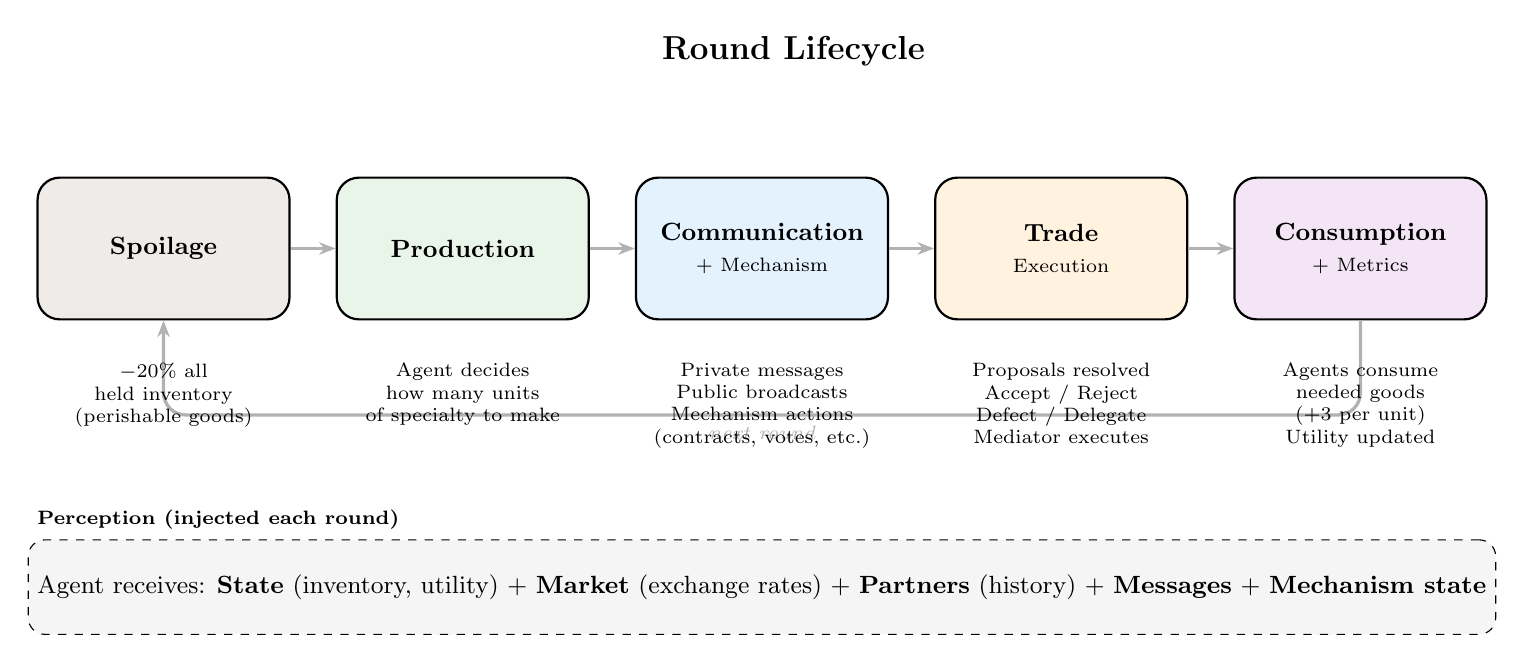
\begin{tikzpicture}[
    phase/.style={draw, rounded corners=8pt, fill=#1!12, minimum width=3.2cm, minimum height=1.8cm, font=\small\bfseries, align=center, thick},
    detail/.style={font=\scriptsize, text width=3cm, align=center},
    arr/.style={-{Stealth[length=6pt]}, very thick, gray!60},
    bigarr/.style={-{Stealth[length=8pt]}, ultra thick, #1!60},
]

% Title
\node[font=\large\bfseries] at (8, 7) {Round Lifecycle};

% Phases in a row
\node[phase=spoil] (p1) at (0, 4.5) {Spoilage};
\node[phase=produce] (p2) at (3.8, 4.5) {Production};
\node[phase=comm] (p3) at (7.6, 4.5) {Communication\\{\scriptsize\normalfont + Mechanism}};
\node[phase=trade] (p4) at (11.4, 4.5) {Trade\\{\scriptsize\normalfont Execution}};
\node[phase=consume] (p5) at (15.2, 4.5) {Consumption\\{\scriptsize\normalfont + Metrics}};

\draw[arr] (p1) -- (p2);
\draw[arr] (p2) -- (p3);
\draw[arr] (p3) -- (p4);
\draw[arr] (p4) -- (p5);

% Loop arrow
\draw[arr, rounded corners=8pt] (p5.south) -- ++(0, -1.2) -| (p1.south)
    node[pos=0.25, below, font=\scriptsize\itshape] {next round};

% Details below each phase
\node[detail, below=12pt of p1] {$-$20\% all\\held inventory\\(perishable goods)};
\node[detail, below=12pt of p2] {Agent decides\\how many units\\of specialty to make};
\node[detail, below=12pt of p3] {Private messages\\Public broadcasts\\Mechanism actions\\{\scriptsize (contracts, votes, etc.)}};
\node[detail, below=12pt of p4] {Proposals resolved\\Accept / Reject\\Defect / Delegate\\Mediator executes};
\node[detail, below=12pt of p5] {Agents consume\\needed goods\\(+3 per unit)\\Utility updated};

% Agent perspective box
\node[draw, dashed, rounded corners=6pt, fill=lightbg, minimum width=14cm, minimum height=1.2cm, font=\small] (agentview) at (7.6, 0.2)
    {Agent receives: \textbf{State} (inventory, utility) + \textbf{Market} (exchange rates) + \textbf{Partners} (history) + \textbf{Messages} + \textbf{Mechanism state}};
\node[font=\scriptsize\bfseries, above=0pt of agentview.north west, anchor=south west] {Perception (injected each round)};

\end{tikzpicture}%
}% end resizebox

\newpage

% ── DIAGRAM 3: Mediation Flow ──
\resizebox{\textwidth}{!}{%
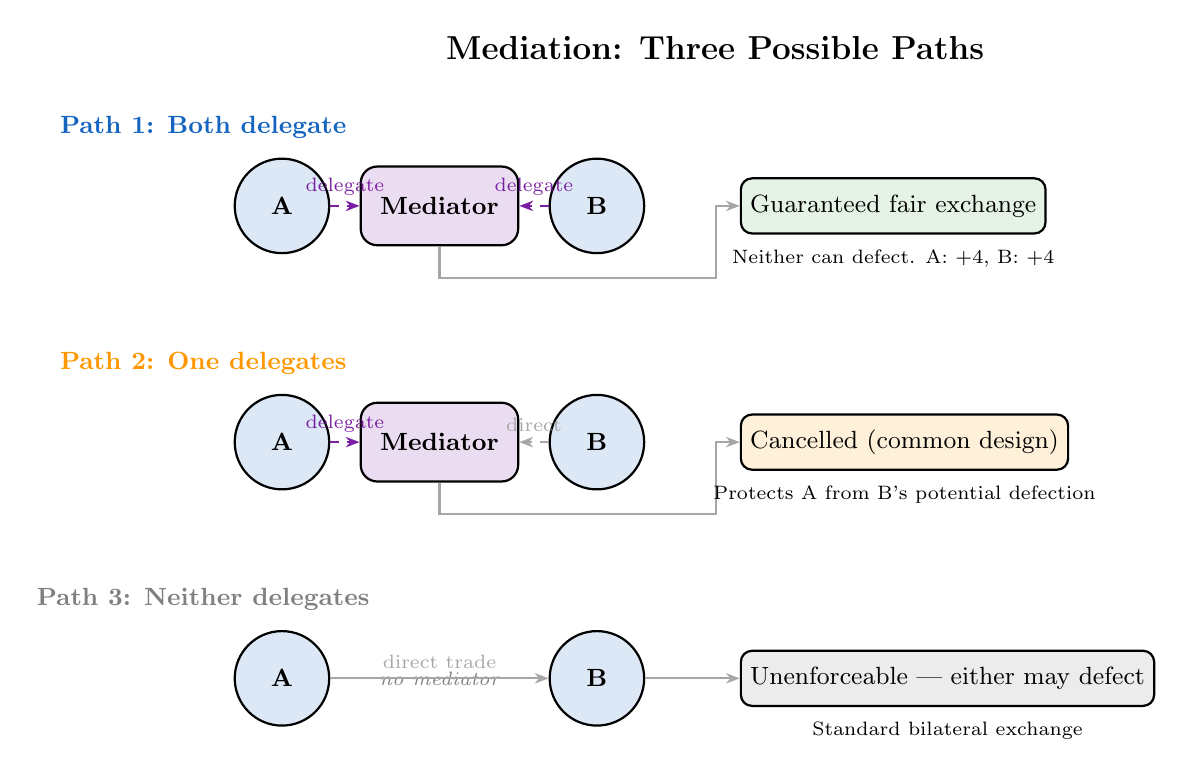
\begin{tikzpicture}[
    agent/.style={draw, circle, fill=honest!15, minimum size=1.2cm, font=\small\bfseries, thick},
    med/.style={draw, rounded corners=6pt, fill=mediator!15, minimum width=2cm, minimum height=1cm, font=\small\bfseries, thick},
    box/.style={draw, rounded corners=5pt, fill=#1!10, minimum width=3cm, minimum height=0.8cm, font=\small, align=center, thick},
    box/.default=gray,
    outcome/.style={draw, rounded corners=4pt, fill=#1!15, minimum width=3.5cm, minimum height=0.7cm, font=\small, align=center, thick},
    arr/.style={-{Stealth[length=5pt]}, thick, gray!70},
    dasharr/.style={-{Stealth[length=5pt]}, thick, dashed, mediator},
]

% Title
\node[font=\large\bfseries] at (5.5, 8.5) {Mediation: Three Possible Paths};

% --- Path 1: Both delegate ---
\node[font=\small\bfseries, honest] at (-1, 7.5) {Path 1: Both delegate};
\node[agent] (a1) at (0, 6.5) {A};
\node[agent] (b1) at (4, 6.5) {B};
\node[med] (m1) at (2, 6.5) {Mediator};
\draw[dasharr] (a1) -- (m1) node[midway, above, font=\scriptsize] {delegate};
\draw[dasharr] (b1) -- (m1) node[midway, above, font=\scriptsize] {delegate};
\node[outcome=produce, right=1.2cm of b1] (out1) {Guaranteed fair exchange};
\draw[arr] (m1.south) -- ++(0, -0.4) -| ($(out1.west)-(0.3,0)$) -- (out1.west);
\node[font=\scriptsize, below=2pt of out1] {Neither can defect. A: +4, B: +4};

% --- Path 2: One delegates ---
\node[font=\small\bfseries, trade] at (-1, 4.5) {Path 2: One delegates};
\node[agent] (a2) at (0, 3.5) {A};
\node[agent] (b2) at (4, 3.5) {B};
\node[med] (m2) at (2, 3.5) {Mediator};
\draw[dasharr] (a2) -- (m2) node[midway, above, font=\scriptsize] {delegate};
\draw[arr, dashed] (b2) -- (m2) node[midway, above, font=\scriptsize] {direct};
\node[outcome=trade, right=1.2cm of b2] (out2) {Cancelled (common design)};
\draw[arr] (m2.south) -- ++(0, -0.4) -| ($(out2.west)-(0.3,0)$) -- (out2.west);
\node[font=\scriptsize, below=2pt of out2] {Protects A from B's potential defection};

% --- Path 3: Neither delegates ---
\node[font=\small\bfseries, gray] at (-1, 1.5) {Path 3: Neither delegates};
\node[agent] (a3) at (0, 0.5) {A};
\node[agent] (b3) at (4, 0.5) {B};
\node[font=\scriptsize\itshape, gray] at (2, 0.5) {no mediator};
\draw[arr] (a3) -- (b3) node[midway, above, font=\scriptsize] {direct trade};
\node[outcome=gray, right=1.2cm of b3] (out3) {Unenforceable --- either may defect};
\draw[arr] (b3) -- (out3);
\node[font=\scriptsize, below=2pt of out3] {Standard bilateral exchange};

\end{tikzpicture}%
}% end resizebox

\newpage

% ── DIAGRAM 4: Progressive Troll Injection Timeline ──
\resizebox{\textwidth}{!}{%
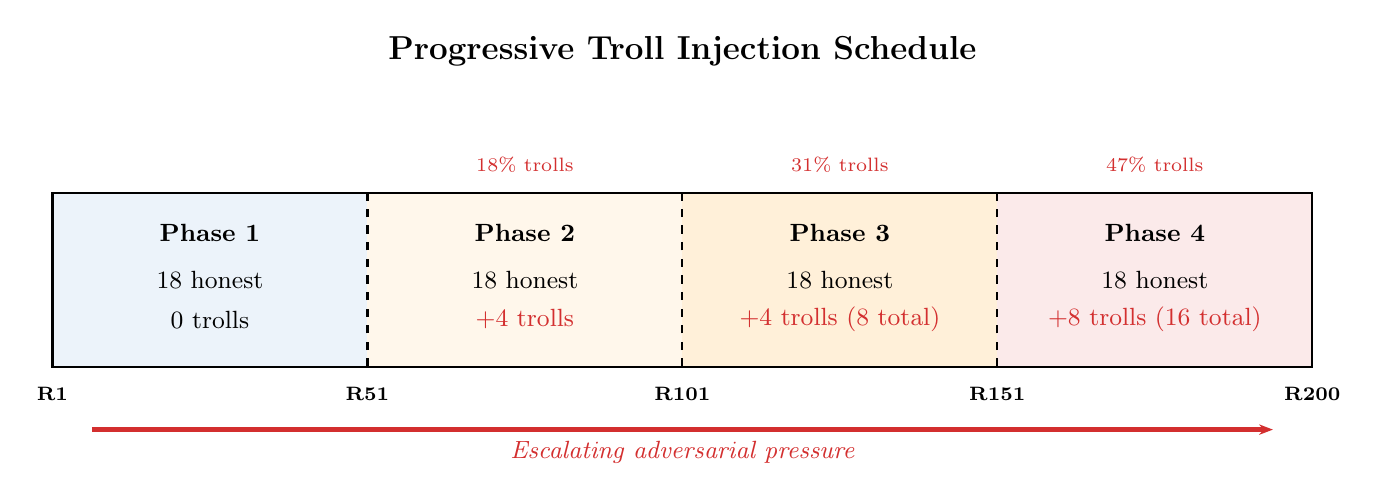
\begin{tikzpicture}[
    phase/.style={draw, rounded corners=6pt, fill=#1!12, minimum height=1.4cm, font=\small, align=center, thick},
    arr/.style={-{Stealth[length=5pt]}, thick, gray!60},
]

% Title
\node[font=\large\bfseries] at (8, 4) {Progressive Troll Injection Schedule};

% Timeline bar
\fill[honest!8] (0, 0) rectangle (4, 2.2);
\fill[trade!8] (4, 0) rectangle (8, 2.2);
\fill[trade!15] (8, 0) rectangle (12, 2.2);
\fill[troll!10] (12, 0) rectangle (16, 2.2);

\draw[thick] (0, 0) rectangle (16, 2.2);
\draw[thick, dashed] (4, 0) -- (4, 2.2);
\draw[thick, dashed] (8, 0) -- (8, 2.2);
\draw[thick, dashed] (12, 0) -- (12, 2.2);

% Phase labels
\node[font=\small\bfseries] at (2, 1.7) {Phase 1};
\node[font=\small\bfseries] at (6, 1.7) {Phase 2};
\node[font=\small\bfseries] at (10, 1.7) {Phase 3};
\node[font=\small\bfseries] at (14, 1.7) {Phase 4};

\node[font=\small] at (2, 1.1) {18 honest};
\node[font=\small] at (2, 0.6) {0 trolls};

\node[font=\small] at (6, 1.1) {18 honest};
\node[font=\small, troll] at (6, 0.6) {+4 trolls};

\node[font=\small] at (10, 1.1) {18 honest};
\node[font=\small, troll] at (10, 0.6) {+4 trolls (8 total)};

\node[font=\small] at (14, 1.1) {18 honest};
\node[font=\small, troll] at (14, 0.6) {+8 trolls (16 total)};

% Round labels
\node[font=\scriptsize\bfseries, below=4pt] at (0, 0) {R1};
\node[font=\scriptsize\bfseries, below=4pt] at (4, 0) {R51};
\node[font=\scriptsize\bfseries, below=4pt] at (8, 0) {R101};
\node[font=\scriptsize\bfseries, below=4pt] at (12, 0) {R151};
\node[font=\scriptsize\bfseries, below=4pt] at (16, 0) {R200};

% Troll percentage
\node[font=\scriptsize, troll, above=4pt] at (6, 2.2) {18\% trolls};
\node[font=\scriptsize, troll, above=4pt] at (10, 2.2) {31\% trolls};
\node[font=\scriptsize, troll, above=4pt] at (14, 2.2) {47\% trolls};

% Arrow showing escalation
\draw[arr, troll, ultra thick] (0.5, -0.8) -- (15.5, -0.8)
    node[midway, below, font=\small\itshape] {Escalating adversarial pressure};

\end{tikzpicture}%
}% end resizebox

\newpage

% ── DIAGRAM 5: Mechanism Taxonomy ──
\resizebox{\textwidth}{!}{%
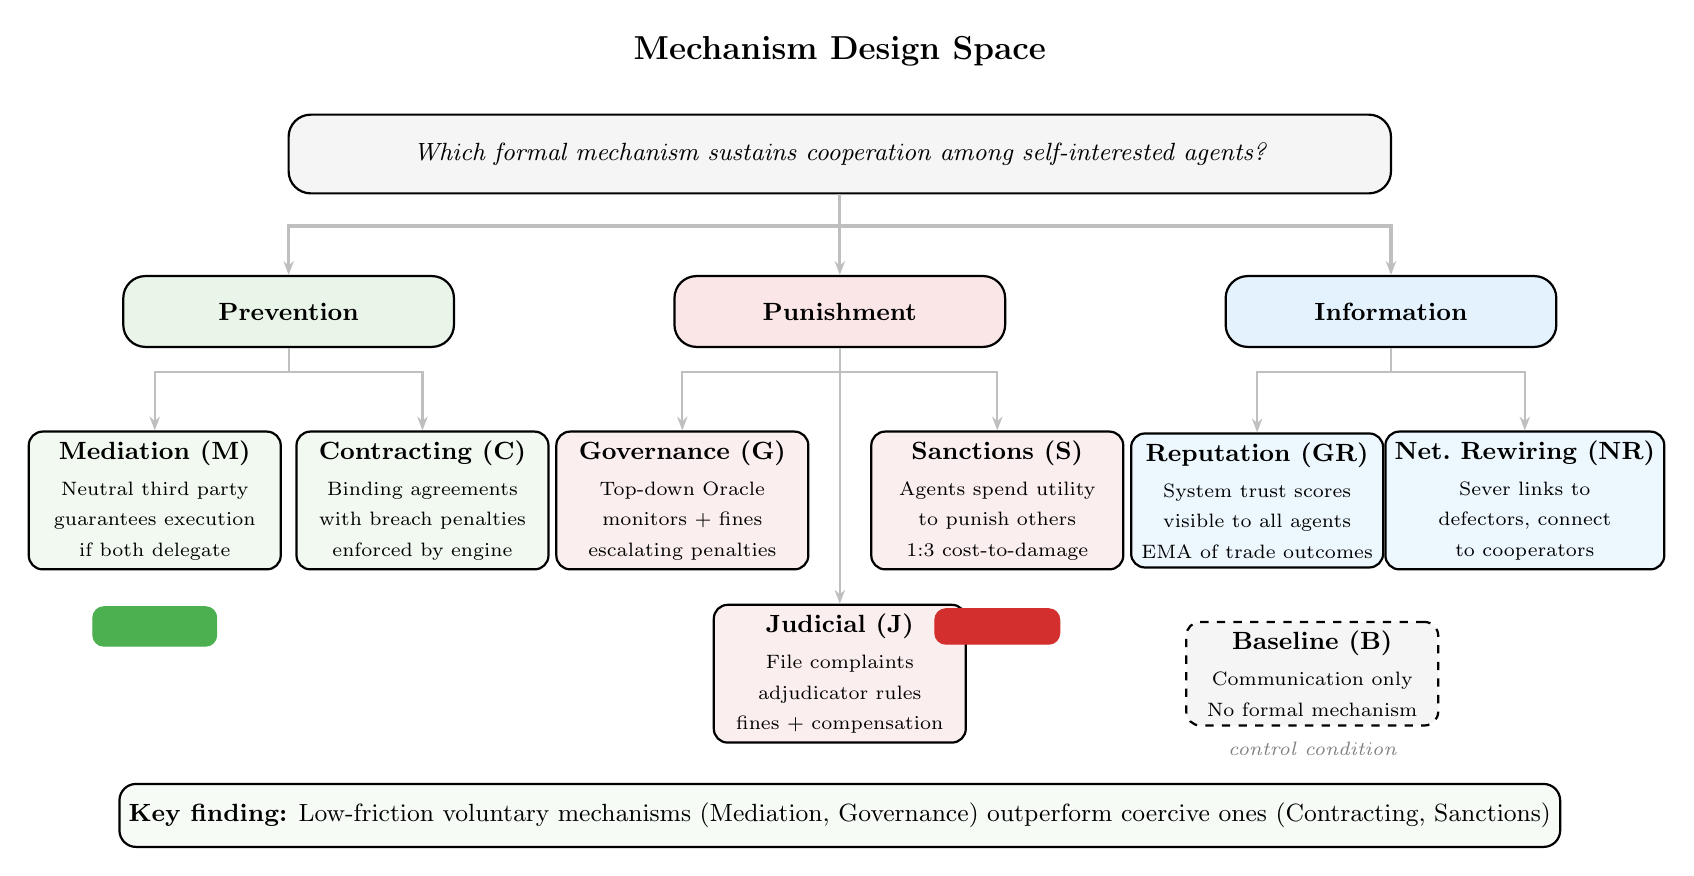
\begin{tikzpicture}[
    cat/.style={draw, rounded corners=8pt, fill=#1!12, minimum width=4.2cm, minimum height=0.9cm, font=\small\bfseries, align=center, thick},
    mech/.style={draw, rounded corners=5pt, fill=#1!8, minimum width=3.2cm, minimum height=1.5cm, font=\small, align=center, thick},
    baseline/.style={draw, rounded corners=5pt, fill=gray!8, minimum width=3.2cm, minimum height=1.2cm, font=\small, align=center, thick, dashed},
    arr/.style={-{Stealth[length=5pt]}, thick, gray!50},
    catarr/.style={-{Stealth[length=5pt]}, very thick, #1!50},
]

% Title
\node[font=\large\bfseries] at (9, 10.5) {Mechanism Design Space};

% Top-level: Research question
\node[draw, rounded corners=8pt, fill=lightbg, minimum width=14cm, minimum height=1cm, font=\small\itshape, align=center, thick] (rq) at (9, 9.2)
    {Which formal mechanism sustains cooperation among self-interested agents?};

% Category headers
\node[cat=produce] (prev) at (2, 7.2) {Prevention};
\node[cat=troll] (pun) at (9, 7.2) {Punishment};
\node[cat=comm] (info) at (16, 7.2) {Information};

\draw[catarr=gray] (rq.south) -- ++(0, -0.4) -| (prev.north);
\draw[catarr=gray] (rq.south) -- (pun.north);
\draw[catarr=gray] (rq.south) -- ++(0, -0.4) -| (info.north);

% Prevention mechanisms
\node[mech=produce] (med) at (0.3, 4.8) {
    \textbf{Mediation (M)}\\[2pt]
    {\scriptsize Neutral third party}\\
    {\scriptsize guarantees execution}\\
    {\scriptsize if both delegate}
};
\node[mech=produce] (con) at (3.7, 4.8) {
    \textbf{Contracting (C)}\\[2pt]
    {\scriptsize Binding agreements}\\
    {\scriptsize with breach penalties}\\
    {\scriptsize enforced by engine}
};

\draw[arr] (prev.south) -- ++(0, -0.3) -| (med.north);
\draw[arr] (prev.south) -- ++(0, -0.3) -| (con.north);

% Punishment mechanisms
\node[mech=troll] (gov) at (7, 4.8) {
    \textbf{Governance (G)}\\[2pt]
    {\scriptsize Top-down Oracle}\\
    {\scriptsize monitors + fines}\\
    {\scriptsize escalating penalties}
};
\node[mech=troll] (san) at (11, 4.8) {
    \textbf{Sanctions (S)}\\[2pt]
    {\scriptsize Agents spend utility}\\
    {\scriptsize to punish others}\\
    {\scriptsize 1:3 cost-to-damage}
};
\node[mech=troll] (jud) at (9, 2.6) {
    \textbf{Judicial (J)}\\[2pt]
    {\scriptsize File complaints}\\
    {\scriptsize adjudicator rules}\\
    {\scriptsize fines + compensation}
};

\draw[arr] (pun.south) -- ++(0, -0.3) -| (gov.north);
\draw[arr] (pun.south) -- ++(0, -0.3) -| (san.north);
\draw[arr] (pun.south) -- (jud.north);

% Information mechanisms
\node[mech=comm] (rep) at (14.3, 4.8) {
    \textbf{Reputation (GR)}\\[2pt]
    {\scriptsize System trust scores}\\
    {\scriptsize visible to all agents}\\
    {\scriptsize EMA of trade outcomes}
};
\node[mech=comm] (nr) at (17.7, 4.8) {
    \textbf{Net.\ Rewiring (NR)}\\[2pt]
    {\scriptsize Sever links to}\\
    {\scriptsize defectors, connect}\\
    {\scriptsize to cooperators}
};

\draw[arr] (info.south) -- ++(0, -0.3) -| (rep.north);
\draw[arr] (info.south) -- ++(0, -0.3) -| (nr.north);

% Baseline
\node[baseline] (base) at (15, 2.6) {
    \textbf{Baseline (B)}\\[2pt]
    {\scriptsize Communication only}\\
    {\scriptsize No formal mechanism}
};
\node[font=\scriptsize\itshape, gray, below=2pt of base] {control condition};

% Result annotations
\node[draw, rounded corners=4pt, fill=produce!15, font=\scriptsize\bfseries, produce, inner sep=4pt] at (0.3, 3.2) {\#1: 1556};
\node[draw, rounded corners=4pt, fill=troll!10, font=\scriptsize\bfseries, troll, inner sep=4pt] at (11, 3.2) {Last: 685};

% Key insight box
\node[draw, rounded corners=6pt, fill=produce!5, minimum width=14cm, minimum height=0.8cm, font=\small, align=center, thick] at (9, 0.8)
    {\textbf{Key finding:} Low-friction voluntary mechanisms (Mediation, Governance) outperform coercive ones (Contracting, Sanctions)};

\end{tikzpicture}%
}% end resizebox

\end{document}
